% Amaya - technical description of the solver.
%
% Compiles with a plain TeX Live installation:  pdflatex amaya && pdflatex amaya
\documentclass[10pt,a4paper]{article}

\usepackage[T1]{fontenc}
\usepackage[utf8]{inputenc}
\usepackage[margin=2.4cm]{geometry}
\usepackage{amsmath}
\usepackage{amssymb}
\usepackage{booktabs}
\usepackage{xcolor}
\usepackage{listings}
\usepackage{tikz}
\usetikzlibrary{positioning,arrows.meta,fit,backgrounds}
\usepackage[hidelinks]{hyperref}

\newcommand{\amaya}{Amaya}
% Allow long identifiers set in \code{} to be hyphenated, so that file paths and symbol
% names do not overflow the text block.
\newcommand{\code}[1]{{\small\ttfamily\hyphenchar\font=`\-\relax #1}}
\newcommand{\Nat}{\mathbb{N}}
\newcommand{\Int}{\mathbb{Z}}

\lstset{
  basicstyle=\ttfamily\footnotesize,
  columns=fullflexible,
  keepspaces=true,
  breaklines=true,
  frame=none,
  xleftmargin=1.5em,
}

\title{\amaya{}: Technical Description of the Solver}
\author{Internal technical report}
\date{Describes the repository state at commit \code{b3fc4d3}, branch \code{devel}}

\emergencystretch=3em
\sloppy

\begin{document}
\maketitle

\section{Purpose, scope, and conventions}
\label{sec:scope}

This document describes the implementation of \amaya{}, an SMT solver for linear integer arithmetic
that decides formulae by constructing finite automata over the binary encoding of integers.  It is a
reference description of the components, algorithms, and configuration options present in the
repository, intended (a) as documentation of what the solver does and (b) as source material for a
subsequent publication.

Scope and method:

\begin{itemize}
  \item Every statement about behaviour is derived from the source at the commit named on the title
        page.  Components that are disabled by default are marked as such at the point of
        description.
  \item Quantitative data appear only in Section~\ref{sec:measurements}.  Their provenance is the
        published SMT-COMP 2025 single-query result dump stored in the repository.  No measurement in
        this document was produced by re-running the solver.
  \item Section~\ref{sec:notmeasured} lists the measurements that a publication would require and
        that are not currently available.
  \item Code is referenced as \code{path:symbol}, e.g.\ \code{amaya/parse.py:\allowbreak evaluate\_\allowbreak exists\_\allowbreak expr}.
        Line numbers are omitted because they are unstable.
  \item Design documents present in the repository are indexed in Section~\ref{sec:docs}; they
        contain the derivations and rationale that this document summarises.
\end{itemize}

\section{Decision procedure}
\label{sec:procedure}

\subsection{Encoding}

The solution domain is $\Int$ (configurable to $\Nat$; see Section~\ref{sec:config}).  A tuple
$(a_1,\dots,a_n) \in \Int^n$ is encoded as a word $w \in (\{0,1\}^n)^{*}$ in the
least-significant-bit-first two's complement encoding: track $i$ of $w$ spells $a_i$ with the least
significant bit first and the sign bit last.  The sign bit may be repeated arbitrarily many times, so
each tuple has infinitely many encodings, and an automaton representing a solution set must accept all
of them.  This property is not preserved by track projection and is restored by the padding closure
(Section~\ref{sec:padclosure}).

Over $\Nat$ the plain binary encoding is used.  The $\Nat$ domain is supported by the native back end
only.

\subsection{Atom types and their automata}

The front end normalises every arithmetic atom into one of three forms
(\code{amaya/relations\_structures.py}):

\begin{center}
\begin{tabular}{llp{72mm}}
\toprule
Type & Form & State space of the constructed automaton \\
\midrule
\code{Relation} (\code{=})  & $\sum_i c_i x_i = k$            & reachable right-hand sides; transition from $k$ on $\sigma$ is $(k - c\cdot\sigma)/2$, undefined if the numerator is odd \\
\code{Relation} (\code{<=}) & $\sum_i c_i x_i \leq k$          & reachable right-hand sides; transition from $k$ on $\sigma$ is $\lfloor (k - c\cdot\sigma)/2 \rfloor$; bounded by $\sum_i |c_i|$ \\
\code{Congruence}           & $\sum_i c_i x_i \equiv k \pmod m$ & residues modulo $m$; at most $m$ states \\
\bottomrule
\end{tabular}
\end{center}

The strict inequality \code{<} is eliminated during normalisation and is never built directly.
Congruences are a first-class atom type rather than being expanded into an existentially quantified
equation; the expansion is available via \code{-p no-congruences} and is required by the LASH export
mode, which has no congruence atom.

The constructions are implemented twice: in Python for the native back end
(\code{amaya/presburger/}) and in C++ for the MTBDD back end
(\code{amaya/mtbdd\_\allowbreak transitions.py:\allowbreak MTBDDTransitionFn.construct\_\allowbreak nfa\_\allowbreak for\_\allowbreak eq}, \code{\dots\_ineq},
\code{\dots\_congruence}).

\subsection{Operations}

Boolean connectives and quantifiers are mapped to automaton operations: conjunction to intersection,
disjunction to union, negation to complementation of a determinised automaton, and existential
quantification to projection of the corresponding track followed by the padding closure.  Universal
quantification is eliminated during normalisation ($\forall = \neg\exists\neg$).  Satisfiability is
decided by searching the resulting automaton for an accepted word
(\code{amaya/mtbdd\_\allowbreak automatons.py:\allowbreak MTBDD\_\allowbreak NFA.find\_\allowbreak model}); a found word is decoded into an integer
assignment by \code{amaya/parse.py:\allowbreak convert\_\allowbreak binary\_\allowbreak model\_\allowbreak into\_\allowbreak decadic}.

\section{Component overview}
\label{sec:overview}

\begin{figure}[t]
\centering
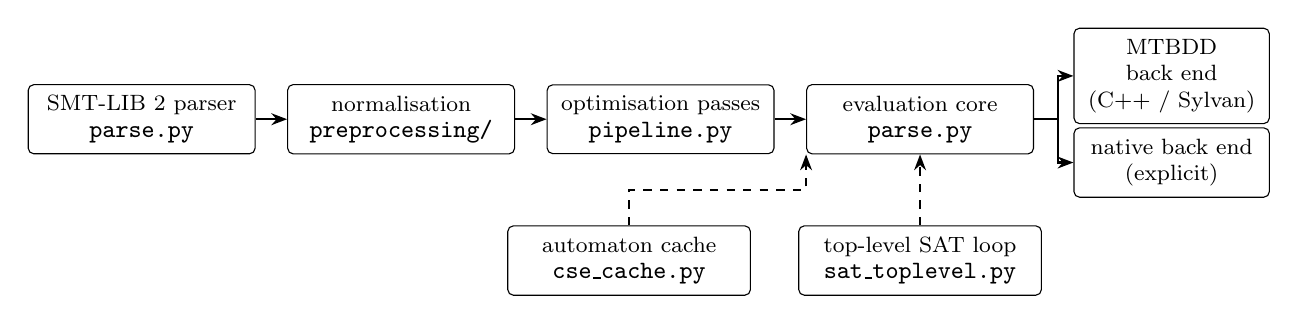
\begin{tikzpicture}[
  node distance=4mm,
  box/.style={draw, rounded corners=2pt, align=center, inner sep=4pt, font=\footnotesize, minimum height=8mm},
  wide/.style={box, text width=26mm},
  arrow/.style={-{Stealth[length=2mm]}, thick},
]
\node[wide] (parse) {SMT-LIB 2 parser\\\code{parse.py}};
\node[wide, right=of parse] (pre) {normalisation\\\code{preprocessing/}};
\node[wide, right=of pre] (opt) {optimisation passes\\\code{pipeline.py}};
\node[wide, right=of opt] (eval) {evaluation core\\\code{parse.py}};

\node[box, right=5mm of eval, text width=22mm, yshift=5.5mm] (mtbdd) {MTBDD back end\\(C++ / Sylvan)};
\node[box, right=5mm of eval, text width=22mm, yshift=-5.5mm] (native) {native back end\\(explicit)};

\node[box, below=9mm of eval, text width=28mm] (sat) {top-level SAT loop\\\code{sat\_toplevel.py}};
\node[box, left=6mm of sat, text width=28mm] (cse) {automaton cache\\\code{cse\_cache.py}};

\draw[arrow] (parse) -- (pre);
\draw[arrow] (pre) -- (opt);
\draw[arrow] (opt) -- (eval);
\draw[arrow] (eval.east) -- ++(3mm,0) |- (mtbdd.west);
\draw[arrow] (eval.east) -- ++(3mm,0) |- (native.west);
\draw[arrow, dashed] (sat) -- (eval);
\draw[arrow, dashed] (cse.north) |- ++(0,4.5mm) -| (eval.south west);
\end{tikzpicture}
\caption{Component structure.  Solid arrows: default execution path.  Dashed: opt-in top-level
strategies that replace or wrap the evaluation core (Sections~\ref{sec:cse} and
\ref{sec:toplevel-sat}); both are disabled by default.}
\label{fig:architecture}
\end{figure}

The solver consists of a Python front end and a C++ automata library
(Figure~\ref{fig:architecture}).  Formula-level processing --- parsing, normalisation, the
optimisation passes, and the scheduling of automaton operations --- is implemented in Python.
Automaton-level processing is implemented in C++ and exposed through a Cython extension
(\code{libamaya}) linked against Sylvan~1.5.

Execution stages:

\begin{enumerate}
  \item \textbf{Parsing} (\code{amaya/tokenize.py}, \code{amaya/parse.py:\allowbreak build\_\allowbreak syntax\_\allowbreak tree}) yields a
        raw S-expression tree.  Top-level statements handled: \code{set-info}, \code{declare-fun},
        \code{assert}, \code{check-sat}, \code{exit}.  Multiple \code{assert} statements are combined
        into a conjunction.  A second \code{check-sat} is rejected.
  \item \textbf{Normalisation} (\code{amaya/preprocessing/\_\allowbreak \_\allowbreak init\_\allowbreak \_\allowbreak .py:\allowbreak preprocess\_\allowbreak ast}) rewrites
        the raw tree and converts it into the typed AST (Section~\ref{sec:frontend}).
  \item \textbf{Optimisation} (\code{amaya/parse.py:\allowbreak optimize\_\allowbreak formula\_\allowbreak structure}) applies the passes
        of Section~\ref{sec:passes} under one of the two coordination strategies of
        Section~\ref{sec:coordination}.
  \item \textbf{Evaluation} (\code{amaya/parse.py:\allowbreak run\_\allowbreak evaluation\_\allowbreak procedure}) walks the optimised AST
        and issues automaton operations to the selected back end (Section~\ref{sec:evalcore}).
  \item \textbf{Answer extraction}: emptiness check and model decoding, or shard-wise model
        composition when sharding is enabled.
\end{enumerate}

\section{Front end}
\label{sec:frontend}

\subsection{Normalisation sequence}

\code{preprocess\_ast} applies the following steps in this order:

\begin{enumerate}
  \item \code{let} macro expansion (\code{expand\_let\_macros}), performed by substitution into the
        body; bindings are expanded innermost-first so that a binding may refer to earlier ones.
  \item If-then-else rewriting (\code{preprocessing/ite\_\allowbreak preprocessing.py:\allowbreak rewrite\_\allowbreak ite\_\allowbreak expressions}).
        ITE terms are lifted out of atoms into a graph of ITE nodes; each node is represented by a
        fresh variable, existentially bound at the atom it originated from, and constrained by the
        branch condition.  The variables introduced here are not formula parameters and are not
        declared in the variable table as such.
  \item $\forall$ elimination (\code{replace\_\allowbreak forall\_\allowbreak with\_\allowbreak exists\_\allowbreak handler}):
        $\forall \vec{x}\,\varphi \mapsto \neg\exists \vec{x}\,\neg\varphi$.
  \item Implication expansion (\code{expand\_implications\_handler}):
        $A \Rightarrow B \mapsto \neg A \vee B$.
  \item Double-negation removal (\code{remove\_\allowbreak double\_\allowbreak negations\_\allowbreak handler}).
  \item Conversion into the typed AST (\code{preprocessing/eval.py:\allowbreak convert\_\allowbreak ast\_\allowbreak into\_\allowbreak evaluable\_\allowbreak form}),
        which produces \code{ASTp\_Node} trees whose leaves are \code{Relation}, \code{Congruence},
        \code{BoolLiteral} and \code{Var}, together with the variable table.
  \item Optional renaming of all variables to generated names
        (\code{assign\_\allowbreak fresh\_\allowbreak names\_\allowbreak to\_\allowbreak all\_\allowbreak vars}), enabled by \code{-p assign-new-var-names}.
\end{enumerate}

\subsection{Variable identity}

\code{preprocessing/eval.py:\allowbreak Scoper} assigns a globally unique integer identity to every bound
variable at conversion time.  Identities are never reused across binders.  Consequences:

\begin{itemize}
  \item No substitution performed by a later pass can capture a variable, and no alpha-conversion pass
        exists in the codebase.
  \item Structural equality of two \code{ASTp\_Node} trees is equality over global identities, not
        alpha-equivalence.  Two subformulae that differ only in the identities of their bound variables
        compare unequal.  Section~\ref{sec:cse} describes the encoding used to recover
        alpha-equivalence where it is needed, and \code{iso-conflicts} (Section~\ref{sec:passes})
        performs an explicit isomorphism check for one specific pattern.
\end{itemize}

The variable table maps \code{Var} to \code{VarInfo} (name, type, and whether the variable is a
formula parameter).  Only formula parameters appear in a reported model.

\subsection{Non-linear terms}

\code{mod}, \code{div}, and products of variables are extracted by
\code{preprocessing/eval.py:\allowbreak normalize\_\allowbreak expr} into a non-linear term graph
(\code{NonlinTermGraph}), whose nodes are keyed by the term body, so that repeated occurrences of the
same term share one node.  Each node is replaced in the atom by a placeholder variable and constrained
by defining relations:

\begin{itemize}
  \item For $t \bmod m$: a remainder variable $r$ with $0 \leq r \leq |m| - 1$, and a decomposition
        $m \cdot d + r = t$ where $d$ is the quotient variable.  The \code{mod} and \code{div} of the
        same body share $d$ and $r$.
  \item By default the decomposition uses one fresh variable; \code{-p nonlinear-term-use-two-vars}
        uses two, which yields smaller automata at the cost of one additional track.
  \item With \code{preprocessing.\allowbreak use\_\allowbreak congruences\_\allowbreak when\_\allowbreak rewriting\_\allowbreak modulo} (default: enabled) the
        \code{mod} constraint is emitted as a \code{Congruence} atom instead of the quantified
        decomposition.
\end{itemize}

Inputs whose non-linear terms fall outside the cases the graph handles are not encoded; the solver
reports \code{unknown} for them.  This is the mechanism by which \amaya{} answers part of the
\code{NIA} division (Section~\ref{sec:measurements}).

\subsection{Typed AST}

\code{ASTp\_Node} is the union of the node types in Table~\ref{tab:astp}.  Internal nodes carry a
\code{referenced\_vars} annotation (the variables occurring in the subtree), which several passes read
instead of re-traversing.  The annotation is invalidated by rewrites that change a subtree and is
refreshed by \code{fill\_referenced\_vars}; the scheduler of Section~\ref{sec:coordination} treats this
refresh as a scheduled repair.

\begin{table}[h]
\centering
\footnotesize
\caption{Node types of the typed AST (\code{amaya/relations\_structures.py}).}
\label{tab:astp}
\begin{tabular}{lp{110mm}}
\toprule
Type & Contents \\
\midrule
\code{Relation}       & \code{vars}, \code{coefs}, \code{rhs}, \code{predicate\_symbol} $\in \{\code{=}, \code{<=}\}$ \\
\code{Congruence}     & \code{vars}, \code{coefs}, \code{rhs}, \code{modulus} \\
\code{BoolLiteral}    & \code{value} \\
\code{Var}            & a Bool-typed variable occurring as an atom \\
\code{AST\_Negation}  & \code{child}, \code{referenced\_vars} \\
\code{AST\_Connective}& \code{type} $\in \{\code{AND}, \code{OR}, \code{EQUIV}\}$, \code{children} ($n$-ary for AND/OR), \code{referenced\_vars} \\
\code{AST\_Quantifier}& \code{bound\_vars}, \code{child}, \code{referenced\_vars}; existential only \\
\bottomrule
\end{tabular}
\end{table}

\subsection{Structural identity}

\code{preprocessing/structural\_\allowbreak id.py:\allowbreak compute\_\allowbreak structural\_\allowbreak id} assigns an integer id to every
subformula from a table keyed by a canonical node key: an atom is keyed by its predicate, right-hand
side, modulus, and the sorted multiset of (variable, coefficient) pairs; a connective by its type and
the sorted multiset of its children's ids.  Two subformulae receive the same id exactly when they are
structurally identical modulo the order of connective children and of the terms within an atom.

A second, distinct traversal exists in
\code{preprocessing/connective\_\allowbreak child\_\allowbreak dedup.py:\allowbreak \_\allowbreak assign\_\allowbreak ids}.  It fuses id assignment with the
deduplication rewrite: it removes duplicate children and collapses single-child connectives, and keys a
connective by a \emph{frozenset} of child ids.  Its ids therefore describe the rewritten tree.  The two
traversals are intentionally not merged: a fingerprint used to detect whether a pass changed the
formula must describe the input tree, otherwise the deduplication pass fingerprints its input and its
output identically and is recorded as unproductive.

\section{Optimisation passes}
\label{sec:passes}

Table~\ref{tab:passes} lists the passes registered in \code{preprocessing/pipeline.py}, the
\code{SolverConfig} field gating each, and the \code{-O} name that enables it.  All fields default to
\code{False} except \code{do\_interval\_analysis} and \code{do\_gcd\_divide}, which default to
\code{True}.  The following subsections state what each pass matches and produces.

\begin{table}[t]
\centering
\footnotesize
\caption{Registered passes (\code{preprocessing/pipeline.py:\allowbreak \_\allowbreak registry\_\allowbreak definition}), in registration
order.  \emph{Tier} is the scheduling priority used by the fixpoint scheduler
(Section~\ref{sec:coordination}), \emph{max} its cap on invocations per pipeline run, and
\emph{growth} the factor beyond which a result is discarded ($\infty$ = no limit).  The \code{-O} name
equals the pass name except where noted.}
\label{tab:passes}
\begin{tabular}{llrrl}
\toprule
Tier & Pass name & max & growth & \code{OptimizationsConfig} field \\
\midrule
normalise & \code{flatten-connectives}       & $\infty$ & $\infty$ & --- (unconditional) \\
normalise & \code{stomp-negations}           & $\infty$ & $\infty$ & \code{push\_negation\_towards\_atoms} \\
normalise & \code{dedup-connective-children} & $\infty$ & $\infty$ & \code{deduplicate\_connective\_children} \\
\midrule
core & \code{var-bounds}              & $\infty$ & $\infty$ & \code{simplify\_variable\_bounds} \\
core & \code{interval-analysis}       & $\infty$ & $\infty$ & \code{do\_interval\_analysis} \\
core & \code{model-reasoning}         & $\infty$ & $\infty$ & \code{reason\_about\_models} \\
core & \code{unconstrained-vars}$^a$  & $\infty$ & $\infty$ & \code{reason\_about\_models} \\
core & \code{inline-bool-definitions} & $\infty$ & $\infty$ & \code{inline\_bool\_var\_definitions} \\
core & \code{rce}                     & $\infty$ & $\infty$ & \code{resolve\_conditional\_equalities} \\
\midrule
heavy & \code{gcd-rewrite}          & 3 & $\infty$ & \code{rewrite\_\allowbreak existential\_\allowbreak equations\_\allowbreak via\_\allowbreak gcd} \\
heavy & \code{infinite-domain}      & 3 & $\infty$ & \code{remove\_\allowbreak vars\_\allowbreak used\_\allowbreak only\_\allowbreak in\_\allowbreak disequalities} \\
heavy & \code{miniscope}            & 2 & 1.5 & \code{do\_miniscoping} \\
heavy & \code{opt-bottom-exists}    & 2 & 1.2 & \code{optimize\_bottom\_quantifiers} \\
heavy & \code{minimize-congruences} & 2 & 1.2 & \code{rewrite\_\allowbreak congruences\_\allowbreak with\_\allowbreak unbound\_\allowbreak terms} \\
heavy & \code{linearize}            & 1 & 1.2 & \code{linearize\_congruences} \\
heavy & \code{iso-conflicts}        & 1 & 1.0 & \code{detect\_isomorphic\_conflicts} \\
heavy & \code{light-sat}            & 1 & 2.0 & \code{do\_light\_sat\_reasoning} \\
\midrule
finalise & \code{finalize-flatten}$^b$ & 1 & $\infty$ & --- (unconditional) \\
finalise & \code{finalize-dedup}$^b$   & 1 & $\infty$ & \code{deduplicate\_connective\_children} \\
finalise & \code{finalize-refvars}$^b$ & 1 & $\infty$ & --- (unconditional) \\
\bottomrule
\multicolumn{5}{l}{\footnotesize $^a$ shares the \code{-O model-reasoning} switch.
  $^b$ finalisers; no \code{-O} name of their own.} \\
\end{tabular}
\end{table}

\subsection{Structural normalisation}

\textbf{\code{flatten-connectives}} (\code{preprocessing/\_\allowbreak \_\allowbreak init\_\allowbreak \_\allowbreak .py:\allowbreak flatten\_\allowbreak bool\_\allowbreak nary\_\allowbreak connectives}).
Merges nested binary AND/OR nodes of the same type into one $n$-ary node and replaces a single-child
AND/OR by its child.  EQUIV nodes are descended into but not merged.  Applied unconditionally, because
downstream passes and the evaluator assume $n$-ary form.

\textbf{\code{stomp-negations}} (\code{preprocessing/unbound\_\allowbreak vars.py:\allowbreak push\_\allowbreak negations\_\allowbreak towards\_\allowbreak atoms}).
Pushes negations towards the leaves using De Morgan's laws.  The evaluator determinises before
complementing, so the position of a negation determines the size of the automaton that is
determinised.

\textbf{\code{dedup-connective-children}}
(\code{preprocessing/connective\_\allowbreak child\_\allowbreak dedup.py:\allowbreak remove\_\allowbreak duplicit\_\allowbreak connective\_\allowbreak children}).
Removes duplicate children of AND/OR/EQUIV using the structural ids described above; detection is
therefore insensitive to the order of children and of the terms within an atom.

\subsection{Bound and interval reasoning}

\textbf{\code{var-bounds}} (\code{preprocessing/unbound\_\allowbreak vars.py:\allowbreak simplify\_\allowbreak bounded\_\allowbreak atoms}).
Computes, bottom-up, an interval abstraction (\code{Value\_Interval}) of the values each variable may
take in each subtree: intersection at AND, union at OR, complementation at NOT.  Atoms settled by the
resulting bounds are rewritten; e.g.\ $x \geq 0 \wedge x \neq 0$ becomes $x \geq 1$, and an atom whose
left-hand side cannot reach its right-hand side becomes a \code{BoolLiteral}.

\textbf{\code{interval-analysis}}
(\code{preprocessing/unbound\_\allowbreak vars.py:\allowbreak prune\_\allowbreak conjunctions\_\allowbreak false\_\allowbreak due\_\allowbreak to\_\allowbreak parent\_\allowbreak context}).
Propagates the assertions of ancestor conjunctions downwards and removes children contradicted by
them.  Example from the source:
\code{(and (>= x 0) (or (and (= x 3) (= y 2)) $\psi$))} loses its first disjunct if an ancestor asserts
$x \leq 2$.  The pass also rewrites relations whose left-hand-side term is bounded by the context
(\code{rewrite\_\allowbreak using\_\allowbreak bounds\_\allowbreak on\_\allowbreak lhs\_\allowbreak lin\_\allowbreak term}).  With \code{purge-twice}
(\code{do\_interval\_reasonining\_twice}) the legacy sequence runs this pass a second time after
quantifier elimination, on the grounds that eliminated quantifiers may expose new constraints.

Interval information is a precondition of two later components: congruence linearisation
(Section~\ref{sec:passes-congruence}) requires finite ranges, and the bounded-congruence construction
(Section~\ref{sec:bounded-congruence}) requires both bounds of the eliminated variable.

\subsection{Quantifier elimination by arithmetic}

\textbf{\code{gcd-rewrite}} (\code{preprocessing/unbound\_\allowbreak vars.py:\allowbreak simplify\_\allowbreak unbounded\_\allowbreak equations}).
Handles a quantifier whose body is a single atom
(\code{\_rewrite\_exists\_equations}):

\begin{itemize}
  \item body is an equation and the quantified variables' coefficients have $\gcd = 1$: the quantifier
        is replaced by $\top$, since the equation is solvable for any value of the remaining terms;
  \item body is an inequation mentioning a quantified variable: replaced by $\top$, since the variable
        can be driven towards the satisfiable side;
  \item body is an inequation not mentioning any quantified variable: the quantifier is dropped.
\end{itemize}

The associated rewrite named in the configuration is
$\exists x\,(k x = y) \mapsto y \equiv 0 \pmod k$, which is one of the reasons congruences are a
first-class atom type.

\textbf{Surjective transformations} (\code{\_\allowbreak rewrite\_\allowbreak surjective\_\allowbreak transformations}, invoked from
\code{opt-bottom-exists}).  Recognises a quantified variable ranging over an interval covered
surjectively by a linear map and replaces the quantifier by the induced constraint.  Implemented case:
$\exists x_1\,(x_1 \geq 0 \wedge x_1 - 5x_2 \in [0,4]) \iff x_2 \geq 0$.  The source lists further
cases as not implemented.

\textbf{\code{opt-bottom-exists}}
(\code{preprocessing/unbound\_\allowbreak vars.py:\allowbreak optimize\_\allowbreak bottom\_\allowbreak quantifiers}).  Operates on quantifiers whose
body is quantifier-free.  It computes a monotonicity abstraction
(\code{\_\allowbreak determine\_\allowbreak monotonicity\_\allowbreak of\_\allowbreak variables}) recording, per variable, whether the solution set of
the body grows as the variable increases, decreases, or both.  A variable that is monotone and
unbounded in the growing direction is instantiated at $\pm\infty$; a variable for which the body
determines a best finite value is instantiated at that value.  In both cases the quantifier is removed
without a projection being performed.

\textbf{\code{infinite-domain}}
(\code{preprocessing/unbound\_\allowbreak vars.py:\allowbreak remove\_\allowbreak vars\_\allowbreak with\_\allowbreak no\_\allowbreak consequences\_\allowbreak on\_\allowbreak the\_\allowbreak model}).  Removes
an existentially quantified variable of an infinite sort that occurs only in disequalities: over $\Int$
a value avoiding finitely many forbidden values always exists.  Example:
$\exists x\,(y \leq 0 \wedge x \neq 5) \mapsto y \leq 0$.

\textbf{Side conditions.}  These rewrites are guarded by conditions the implementations check
explicitly.  The sharpest is in \code{unconstrained-vars} below: an equation may be dropped because one
of its variables occurs nowhere else only when the $\gcd$ of the coefficients of such variables is~1.
For instance $3x + z = 3$ conjoined with $z \leq 0$ has no integer solution although $z$ occurs nowhere
else.  Inequations require no such condition, because any non-zero coefficient allows the variable to
be driven to $\pm\infty$.

\subsection{Congruence rewriting}
\label{sec:passes-congruence}

\textbf{\code{minimize-congruences}}
(\code{preprocessing/unbound\_\allowbreak vars.py:\allowbreak simplify\_\allowbreak congruences\_\allowbreak on\_\allowbreak unbounded\_\allowbreak existential\_\allowbreak vars}).
Matches an $\exists$-quantified conjunction in which some bound variables occur only inside
congruences.  A group of such variables that enters a congruence only through a linear combination is
replaced by a single fresh variable whose coefficient is the $\gcd$ of the group's coefficients:
$a x + b y \equiv k$ with $x, y$ unconstrained elsewhere becomes
$a x + \gcd(b, \dots)\, y' \equiv k$.  This reduces the number of tracks in the resulting automaton.

\textbf{\code{linearize}} (\code{preprocessing/unbound\_\allowbreak vars.py:\allowbreak linearize\_\allowbreak congruences}).  Matches a
congruence over exactly two variables whose ranges are finite --- either explicitly bounded, or
implicitly bounded because the monotonicity abstraction fixes the relevant side --- and replaces it by
linear constraints with the same solution set (\code{\_\allowbreak attempt\_\allowbreak congruence\_\allowbreak linearization}).  The pass
estimates the stride of the relation (\code{\_should\_linearize}) before committing and declines
otherwise.  The intended profitable case is a modulus large relative to the variables' ranges.

\subsection{Structural rewrites}

\textbf{\code{miniscope}} (\code{preprocessing/antiprenexing.py:\allowbreak miniscope\_\allowbreak quantifiers}).  Pushes each
quantifier towards the leaves as far as its bound variables allow: adjacent quantifier blocks are
merged, a quantified conjunction is split into the conjuncts mentioning the variable and those not
mentioning it, and a quantified disjunction is distributed.  Quantifiers are not pushed through
negations or EQUIV nodes.  Two consequences for the evaluator: the projection is performed on the
smallest automaton still mentioning the variable, and the resulting shape --- an existentially
quantified conjunction of atoms --- is the input pattern of the lazy construction
(Section~\ref{sec:lazy}) and of the bounded-congruence construction
(Section~\ref{sec:bounded-congruence}).

\textbf{\code{inline-bool-definitions}}
(\code{preprocessing/unbound\_\allowbreak vars.py:\allowbreak inline\_\allowbreak bool\_\allowbreak var\_\allowbreak definitions}).  Collects equivalences
$b \leftrightarrow \varphi$ that hold unconditionally --- reachable from the root through conjunctions
and quantifiers only, never through a disjunction or an EQUIV, where they would hold only within one
branch --- substitutes $\varphi$ for every occurrence of $b$, and removes the defining equivalence.
Example: \code{(and (= b (or x y)) (or b z))} becomes \code{(or x y z)}.  Variables with conflicting
definitions are excluded, and cyclic definitions are detected during resolution.

\textbf{\code{rce}} (\code{preprocessing/conditional\_\allowbreak equality\_\allowbreak resolution.py}).  Eliminates an
existentially quantified variable occurring only in equalities inside disjunctions:
\[
  \exists x \bigwedge_{i=1}^{n}(\alpha_i \vee x = t_i)
  \;\iff\;
  \bigvee_{i=1}^{n} \alpha_i \;\vee\; \bigvee_{1 \leq i < j \leq n} t_i = t_j .
\]
Preconditions checked by the implementation: the body is a conjunction of disjunctions; $x$ occurs
exactly once per clause, in an equality with unit coefficient on $x$; $x$ does not occur in any escape
literal $\alpha_i$ or term $t_i$; the sort of $x$ is infinite.  The pattern occurs in formulae produced
by verification tools that encode $\phi$-nodes of a program's control flow.

\textbf{\code{model-reasoning}} (\code{preprocessing/theory\_\allowbreak reasoning.py:\allowbreak \allowbreak
simplify\_\allowbreak formula\_\allowbreak using\_\allowbreak model\_\allowbreak properties}).  Traverses the formula while maintaining
\code{Asserted\_Model\_Properties}: the equations, Boolean atom values and variable aliases
($x = \sum_i c_i y_i + c$) that hold on the current branch.  Facts are used to simplify the subtree
below: a variable with a known alias is substituted away, an implied atom is replaced by $\top$, and a
congruence made unsatisfiable by the substitution is replaced by $\bot$.  The structure records, per
fact, the branch depth and the negation depth at which it was learned, and the stack of open
quantifiers; a fact learned at a negation depth different from that of its enclosing connective is not
implied by that branch and is not retained, and facts learned inside a quantifier body are discarded on
leaving it.

\textbf{\code{unconstrained-vars}}
(\code{preprocessing/theory\_\allowbreak reasoning.py:\allowbreak remove\_\allowbreak atoms\_\allowbreak satisfied\_\allowbreak by\_\allowbreak unconstrained\_\allowbreak vars}).  Uses a
variable-use scan to identify variables occurring in exactly one atom, and removes atoms that such a
variable can always satisfy.  For equations, the pass requires $\gcd$ of the unconstrained variables'
coefficients to be~1 (see the side condition above); inequations are unconditional.

\textbf{\code{iso-conflicts}}
(\code{preprocessing/unbound\_\allowbreak vars.py:\allowbreak detect\_\allowbreak conflics\_\allowbreak on\_\allowbreak isomorphic\_\allowbreak fragments}).  Detects
$\varphi \wedge \neg\varphi'$ among the children of a conjunction where $\varphi$ and $\varphi'$ are
isomorphic modulo renaming of bound variables, and replaces the conjunction by $\bot$.  This closes a
gap created by the globally-unique-identity scheme, under which such pairs are not syntactically equal.
The isomorphism check (\code{are\_\allowbreak exists\_\allowbreak and\_\allowbreak trees\_\allowbreak isomorphic}) is an under-approximation: it fixes
free variables and attempts one variable correspondence.

\textbf{\code{light-sat}}
(\code{preprocessing/unbound\_\allowbreak vars.py:\allowbreak convert\_\allowbreak and\_\allowbreak or\_\allowbreak trees\_\allowbreak to\_\allowbreak dnf\_\allowbreak if\_\allowbreak talking\_\allowbreak about\_\allowbreak similar\_\allowbreak atoms}).
Converts two-level AND-OR trees into DNF when the inner disjunctions mention a subset of the atoms of
the enclosing conjunction, and detects contradictory clauses.  It has the largest growth factor of any
pass (2.0) and a run cap of 1.

\section{Coordination of the passes}
\label{sec:coordination}

Two coordination strategies exist.  \code{amaya/parse.py:\allowbreak optimize\_\allowbreak formula\_\allowbreak structure} dispatches on
\code{solver\_\allowbreak config.\allowbreak optimization\_\allowbreak pipeline.\allowbreak enabled}.

\subsection{Legacy sequence (default)}

\code{\_\allowbreak optimize\_\allowbreak formula\_\allowbreak structure\_\allowbreak legacy} applies the enabled passes in a fixed, hand-unrolled
order:

\begin{enumerate}
  \item \code{var-bounds};
  \item \code{gcd-rewrite};
  \item \code{minimize-congruences};
  \item \code{stomp-negations};
  \item \code{flatten-connectives};
  \item \code{iso-conflicts};
  \item \code{light-sat};
  \item \code{interval-analysis};
  \item \code{miniscope};
  \item \code{opt-bottom-exists};
  \item \code{linearize};
  \item \code{interval-analysis} again, if \code{purge-twice};
  \item \code{model-reasoning} twice, then \code{unconstrained-vars} three times;
  \item \code{inline-bool-definitions};
  \item \code{infinite-domain} twice;
  \item \code{model-reasoning} twice again;
  \item \code{rce} interleaved with \code{flatten-connectives}, ten applications in total, with one
        \code{miniscope} in the middle;
  \item \code{dedup-connective-children} followed by \code{flatten-connectives}.
\end{enumerate}

The repeated applications encode, by repetition, the dependencies between passes: each application
waits for the preceding one to expose new structure.  The repetition counts are fixed and are not
derived from the formula.

\subsection{Fixpoint scheduler (opt-in)}

\code{preprocessing/pipeline.py:\allowbreak Optimization\_\allowbreak Pipeline} replaces the fixed order with a scheduler.
Each pass is registered as a \code{Pass\_Descriptor} with the following fields:

\begin{center}
\footnotesize
\begin{tabular}{lp{104mm}}
\toprule
Field & Meaning \\
\midrule
\code{name}                & stable identifier, used in reports and in the tier/max-run overrides \\
\code{config\_flag}        & \code{OptimizationsConfig} attribute gating the pass; \code{None} = unconditional \\
\code{tier}                & scheduling priority: normalise (0), core (1), heavy (2), finalise (3) \\
\code{consumes}            & structural facts whose (re)appearance makes the pass worth re-running \\
\code{produces}            & structural facts the pass may create when it fires \\
\code{max\_runs}           & cap on invocations per pipeline run \\
\code{growth\_factor\_limit} & factor above which the pass's result is discarded \\
\code{needs\_referenced\_vars} & whether \code{fill\_referenced\_vars} must run first \\
\code{self\_triggering}    & whether a productive run re-enqueues the pass itself (default: true) \\
\bottomrule
\end{tabular}
\end{center}

Scheduling rule: passes are popped by \code{(tier, registration index)}; a productive run enqueues
every pass whose \code{consumes} set intersects the run's \code{produces} set, plus the pass itself if
\code{self\_triggering}.  A single persistent \code{Structural\_Id\_Table} is used for change detection,
so a pass whose output fingerprints identically to its input is recorded as unproductive and does not
trigger anything.  Termination conditions:

\begin{itemize}
  \item \textbf{Fixpoint}: the queue empties.  The current formula is returned.
  \item \textbf{Cycle}: a formula fingerprint repeats, i.e.\ some set of passes is undoing each other's
        work.  The best formula seen is returned.
  \item \textbf{Budget}: \code{max\_pass\_applications} is exhausted.  Default is derived from formula
        size (32 applications per 1000 nodes, clamped to $[256, 512]$).  The best formula is returned.
  \item \textbf{Time}: \code{max\_wall\_time\_seconds} is exceeded (0 = no limit).  The best formula is
        returned.
\end{itemize}

The score of a formula is the pair (node count, quantifier count), lexicographically.  A pass whose
result exceeds its growth factor has that result discarded but is still charged an invocation.
Finalisers (tier 3) run once, after the main loop, in registration order.

The scheduler is disabled by default (\code{--opt-fixpoint} enables it, \code{--no-opt-fixpoint}
forces the legacy path); \code{--opt-budget} overrides the budget and \code{--opt-report} logs a
per-pass table of invocations, productive runs, growth discards, time, and nodes removed.  The
differential validation of the scheduler against the legacy sequence is incomplete; see
\code{PROGRESS.md} in the repository.

\section{Evaluation core}
\label{sec:evalcore}

\code{amaya/parse.py:\allowbreak run\_\allowbreak evaluation\_\allowbreak procedure} dispatches on the node type and returns an automaton
for the subformula.  \code{amaya/solver\_\allowbreak core.py:\allowbreak EvaluationContext} carries the alphabet, the variable
table, the automaton class of the selected back end, and the statistics trace.

\begin{center}
\footnotesize
\begin{tabular}{ll}
\toprule
Node & Handler \\
\midrule
\code{Relation}        & \code{build\_\allowbreak automaton\_\allowbreak from\_\allowbreak presburger\_\allowbreak relation\_\allowbreak ast} \\
\code{Congruence}      & \code{make\_nfa\_for\_congruence} (variables sorted, right-hand side normalised modulo $m$) \\
\code{BoolLiteral}     & \code{trivial\_accepting} / \code{trivial\_nonaccepting} \\
\code{Var}             & \code{build\_\allowbreak automaton\_\allowbreak for\_\allowbreak boolean\_\allowbreak variable} \\
\code{AST\_Connective} & \code{evaluate\_and\_expr} / \code{evaluate\_or\_expr} / \code{evaluate\_bool\_equivalence\_expr} \\
\code{AST\_Negation}   & \code{evaluate\_not\_expr} (determinise, then complement) \\
\code{AST\_Quantifier} & \code{evaluate\_exists\_expr} \\
\bottomrule
\end{tabular}
\end{center}

Details of the handlers:

\begin{itemize}
  \item \textbf{Conjunction and disjunction} share
        \code{evaluate\_\allowbreak binary\_\allowbreak conjunction\_\allowbreak expr}, which folds the children with intersection or
        union.  For conjunctions the children are first reordered by
        \code{reorder\_\allowbreak conjunction\_\allowbreak to\_\allowbreak derive\_\allowbreak conflict\_\allowbreak more\_\allowbreak quickly}: children are sorted by an
        \emph{a priori} size estimate ($\sum_i |c_i|$ for a relation, $|m|$ for a congruence, twice that
        under a negation) and then grouped so that consecutive children share variables, so that a
        conflict, if present, appears after few intersections.
  \item \textbf{Equivalence} is evaluated as
        $(\neg L \vee R) \wedge (\neg R \vee L)$ and is restricted to two children.
  \item \textbf{Existential quantification} projects the bound variables one at a time.  The padding
        closure is skipped for all but the last projected variable of a quantifier block
        (\code{do\_\allowbreak projection(var, skip\_\allowbreak pad\_\allowbreak closure=.\allowbreak .\allowbreak .\allowbreak )}), since it is only required once the whole
        block has been eliminated.  Before the generic path, two specialised constructions are
        attempted when enabled: the bounded-congruence construction and the lazy construction
        (Section~\ref{sec:constructions}).
  \item \textbf{Minimisation} is applied at points chosen by
        \code{minimize\_\allowbreak automaton\_\allowbreak if\_\allowbreak configured}: after complementation, after quantification, and
        after each lazily constructed conjunction.  The method is \code{NONE} by default;
        \code{--fast} or \code{-m hopcroft} selects Hopcroft minimisation (which determinises first if
        needed); Brzozowski minimisation is available on the native back end only.
\end{itemize}

\paragraph{Answer extraction.}
\code{evaluate\_\allowbreak prepared\_\allowbreak formula\_\allowbreak with\_\allowbreak automata} builds the automaton for the whole formula, runs
\code{find\_model} (a breadth-first search for an accepted word, which over $\Int$ requires a non-empty
word), and decodes the word into an assignment of the formula parameters.  The function is a parameter
of \code{perform\_\allowbreak whole\_\allowbreak evaluation\_\allowbreak on\_\allowbreak source\_\allowbreak text}, which is how the top-level SAT driver
(Section~\ref{sec:toplevel-sat}) replaces this step while sharing parsing, preprocessing, and context
setup.

\paragraph{Sharding.}
When \code{--shard} is given and the root is a conjunction, \code{split\_conjunction\_to\_shards}
partitions the conjuncts into variable-disjoint groups by union-find over the variables, and
\code{evaluate\_using\_sharding} decides each group independently, intersecting incrementally and
minimising after each step.  An empty group language terminates the run with \code{unsat}; otherwise
the per-group models are concatenated.

\paragraph{Instrumentation.}
Every operation is bracketed by \code{stats\_operation\_starts}/\code{stats\_operation\_ends}, which
record the operation type (\code{amaya/stats.py:\allowbreak ParsingOperation}), the operand and result sizes, and
optionally the runtime, and invoke the introspection handle used by the automaton export.  The same
hook enforces \code{--max-states}: an intermediate automaton exceeding the limit terminates the run.

\section{Automata back ends}
\label{sec:backend}

Two back ends implement the same interface (\code{amaya/automatons.py:\allowbreak NFA} and
\code{amaya/mtbdd\_\allowbreak automatons.py:\allowbreak MTBDD\_\allowbreak NFA}).

\subsection{Native back end}

Transitions are stored as explicit symbol tuples over the whole alphabet
(\code{amaya/transitions.py}).  The back end supports state-semantics tracking
(\code{amaya/semantics\_tracking.py}): each macrostate records the conjunction of atom right-hand sides
it represents, which is used when exporting and inspecting intermediate automata.  It supports both
solution domains and both minimisation methods.  It is the default back end
(\code{--backend native}) and is the slower of the two.

\subsection{MTBDD back end: representation}

The transition function of a state is a Sylvan MTBDD over the automaton's variables, mapping a symbol
in $\{0,1\}^n$ to a set of successor states.  An automaton is a map from state to MTBDD, plus the
initial and final state sets and the BDD variable set (\code{mtbdd-backend/include/base.hpp:\allowbreak NFA}).
Three custom leaf types are registered with Sylvan, each supplying create, destroy, equality, hash and
print callbacks (\code{mtbdd-backend/include/custom\_\allowbreak leaf.hpp}):

\begin{itemize}
  \item \textbf{set leaf}: a sorted vector of destination states (\code{Transition\_Destination\_Set});
  \item \textbf{bit-set leaf}: a fixed-width bitmap of states, used by the padding closure;
  \item \textbf{singleton leaf}: a single state.
\end{itemize}

Two properties of the representation are used by the algorithms below.  First, an automaton's variable
set is narrow: an atom's automaton is built over the atom's own variables
(\code{mtbdd\_transitions.py}), a union widens to the union of the operands' variables, and a
projection removes one.  Second, Sylvan hash-conses its nodes, so structurally identical MTBDDs are the
same pointer and equality of transition functions is a pointer comparison.

\subsection{MTBDD back end: operations}

Each operation is implemented as an MTBDD \emph{apply} --- a memoised traversal of one or two MTBDDs
--- with the operation-specific logic in the leaf case
(\code{mtbdd-backend/src/operations.cpp}, \code{mtbdd-backend/src/base.cpp}).

\paragraph{Intersection} (\code{compute\_nfa\_intersection}, \code{transitions\_intersection2\_op}) is
an on-the-fly product construction.  A work queue holds discovered product states.  For each product
state, the operands' transition MTBDDs are applied against each other; at a pair of leaves the
operator forms the product of the two destination sets, allocates a handle for each product pair not
seen before, pushes newly discovered pairs onto the queue, and returns a leaf containing the handles.
Only reachable product states are constructed.  Two prunings are applied: a product state in which one
component has no outgoing transitions and which is not accepting is skipped
(\code{skip\_\allowbreak product\_\allowbreak state\_\allowbreak due\_\allowbreak to\_\allowbreak no\_\allowbreak post}), and states from which no final state is reachable are
removed afterwards (\code{remove\_nonfinishing\_states}).  Both are compile-time switchable.

\paragraph{Determinisation} (\code{determinize\_nfa}) is the macrostate construction.  The transition
MTBDD of a macrostate is the union of its members' MTBDDs, computed by an apply whose leaf case unions
destination sets; a second, unary apply (\code{replace\_\allowbreak macrostates\_\allowbreak with\_\allowbreak handles\_\allowbreak op}) rewrites the
leaves of that union --- which contain sets of original states --- into macrostate handles, discovering
new macrostates as it proceeds.  A trap state is allocated speculatively and retained only if some
symbol has no successor.

\paragraph{Complementation} swaps final and non-final states of a complete DFA; completion against a
trap state is performed by \code{complete\_with\_trap\_state} when needed.

\paragraph{Projection} (\code{project\_\allowbreak variable\_\allowbreak away\_\allowbreak abstract\_\allowbreak op}) abstracts the variable from the
MTBDD with an operator that unions the leaves reachable along both branches of the abstracted variable.

\subsection{Padding closure}
\label{sec:padclosure}

Projection can remove accepting runs that existed only for a particular padding of the projected
track, so the automaton must be closed under repetition of the sign bit again.  The closure makes final
every state from which a final state is reachable by reading padding symbols only, and adds the
corresponding transitions.

\code{NFA::perform\_pad\_closure} computes this as a fixpoint over a \emph{frontier} MTBDD:

\begin{enumerate}
  \item The frontier is initialised to a leaf containing the final states.
  \item Each round applies every state's transition MTBDD against the current frontier with
        \code{build\_pad\_closure\_frontier\_op}, which adds the origin state wherever the transition
        enters the frontier along a padding symbol.
  \item Rounds repeat until the frontier MTBDD is unchanged; the test is a pointer comparison.
  \item A second sweep applies each state's transitions against the converged frontier
        (\code{add\_pad\_transitions\_op}), adding transitions into one fresh final state where
        required.  The fresh state is added to the automaton only if some transition was added.
\end{enumerate}

The frontier changes on nearly every apply, so its representation determines the cost of the loop.  The
bit-set leaf (\code{mtbdd-backend/include/bit\_\allowbreak set.hpp}) makes each leaf update a fixed-width word copy
rather than a copy and re-sort of a growing sorted vector.  Two implementation constraints are recorded
in the source: (i) each bit set carries its own \code{block\_cnt} rather than reading the allocator's
current generation, because Sylvan owns the leaves and may hash, compare or destroy one after its
generation has ceased to be current; and (ii) each bit set carries a \code{state\_bias}, the smallest
state number of its generation, because \amaya{}'s state numbers are arbitrary signed integers --- a
state derived from an inequation's right-hand side is frequently negative --- while bit indices are
not.  Sets are allocated from a block arena
(\code{mtbdd-backend/include/block\_\allowbreak allocator.h}) in generations sized per automaton.  The
representation is selected by \code{--use-bit-sets} /
\code{BackendConfig.\allowbreak use\_\allowbreak bit\_\allowbreak set\_\allowbreak pad\_\allowbreak closure} (default: enabled in the config dataclass).

\subsection{Minimisation}

\code{minimize\_hopcroft} performs partition refinement.  The initial partition is (final, non-final).
Each round rewrites every state's transition MTBDD with a unary apply
(\code{replace\_\allowbreak states\_\allowbreak with\_\allowbreak partition\_\allowbreak ids\_\allowbreak op}) that replaces each destination state in a leaf by the
id of its current partition, and groups states by the pair (resulting MTBDD, previous partition id).
Because Sylvan hash-conses, two states fall into the same group exactly when their partition-mapped
transition MTBDDs are the same node, so the refinement step is a hash-table insertion keyed on a
pointer.  Rounds repeat until the number of classes stops increasing; the result is assembled from the
MTBDDs computed in the last round.

Three cases are handled explicitly: an automaton with no final states yields a one-state automaton with
a universal self-loop (not a zero-state automaton, which downstream operations do not accept); an
automaton all of whose states are final yields the two-state accept-all automaton; and states
unreachable in the result are removed, because partition refinement processes every state regardless of
reachability while the native back end's minimiser explores only reachable partitions.

\subsection{Renaming, memory management, interruption, binding}

\textbf{Renaming.}  \code{rename\_vars} renames the automaton's tracks.  The renaming must be strictly
monotone on the automaton's variables; a non-monotone renaming raises \code{std::invalid\_argument},
because it would violate the MTBDD variable order rather than fail visibly.  This constraint determines
the variable numbering used by the automaton cache (Section~\ref{sec:cse}).

\textbf{Memory.}  Sylvan is reference-counted and the front end is garbage-collected.  The invariant
maintained by the back end is that every MTBDD reachable from an automaton handed to Python is
referenced once by that automaton, and that each operation references its output independently of its
inputs, so that Python's collector decrements the two independently.  Intermediate MTBDDs inside apply
loops are referenced and dereferenced in step, which bounds node-table growth in fixpoint loops such as
the padding closure.  The lazy construction adds a separate slab allocator and hash-consed pool for
formulae (Section~\ref{sec:lazy}).

\textbf{Interruption.}  Long-running loops in C++ are guarded by \code{Interrupt\_Guard}
(\code{mtbdd-backend/include/interrupt.hpp}) and poll an interrupt flag
(\code{AMAYA\_CHECK\_INTERRUPT}), so that a signal delivered during a long intersection, determinisation
or closure is honoured rather than deferred until the call returns.

\textbf{Binding.}  The back end is compiled into a Cython extension, \code{libamaya}
(\code{mtbdd-backend/wrapper/}), linked against Sylvan~1.5.  It replaces an earlier \code{ctypes}
interface that marshalled state sets across the boundary on every call.

\section{Specialised constructions}
\label{sec:constructions}

\subsection{Lazy construction with formula entailment}
\label{sec:lazy}

\code{mtbdd-backend/src/lazy.cpp} constructs the automaton for a formula
$\exists \vec{y}\,(A_1 \wedge \dots \wedge A_k)$ in one exploration, without constructing the
intersection $\mathcal{A}(A_1) \cap \dots \cap \mathcal{A}(A_k)$.  Entry points:
\code{MTBDDTransitionFn.\allowbreak construct\_\allowbreak dfa\_\allowbreak for\_\allowbreak atom\_\allowbreak conjunction}, called from
\code{amaya/parse.py:\allowbreak try\_\allowbreak lazy\_\allowbreak construct\_\allowbreak conjunction} (whole quantified conjunction) and from
\code{evaluate\_\allowbreak binary\_\allowbreak conjunction\_\allowbreak expr} (the atom-only part of a mixed conjunction, selected by
\code{select\_\allowbreak children\_\allowbreak to\_\allowbreak lazily\_\allowbreak evaluate} when the atoms' variable density exceeds 0.5).

\textbf{State representation.}  A state of the constructed automaton is a macrostate: a set of pairs
$(\varphi, \vec{k})$ where $\varphi$ is a quantified conjunction of atoms
(\code{Quantified\_Atom\_Conjunction}) and $\vec{k}$ assigns a right-hand side to each atom
(\code{Conjunction\_State}).  Macrostates are finalised into a canonical form
(\code{Finalized\_Macrostate}: sorted formula headers plus serialised state data) so that they can be
compared and hashed by memory contents.

\textbf{Successor computation} (\code{explore\_macrostate}).  For each transition symbol over the free
variables, the quantified bits are enumerated (\code{Alphabet\_Iterator}) and the successors of every
pair are collected into one post-macrostate; this performs the projection during construction.  Four
mechanisms bound the size of the result:

\begin{enumerate}
  \item \textbf{Entailment (Pareto) pruning} (\code{find\_pareto\_optimal\_position}).  Within a
        macrostate, a pair whose inequation right-hand sides are pointwise dominated by another pair
        with the same equation and congruence values has a contained language and is discarded.
        Post-states are stored as a Pareto frontier bucketed by the (equation, congruence) prefix and
        kept in sorted order, which also yields the canonical macrostate representation.
  \item \textbf{Contradiction detection} (\code{detect\_contradictions}).  Each formula carries a
        dependency graph (\code{Dep\_Graph}) recording, per variable, the inequations bounding it from
        above and below, the equations and congruences mentioning it, and which of these are hard
        bounds.  Successors whose bounds are contradictory are discarded.
  \item \textbf{On-the-fly formula rewriting} (\code{perform\_watched\_rewrites},
        \code{mtbdd-backend/src/rewrites.cpp}).  When the right-hand sides reached during exploration
        enable a simplification, the successor's formula is rewritten: variables with a known value are
        substituted (\code{substitute\_\allowbreak vars\_\allowbreak with\_\allowbreak known\_\allowbreak value}), quantified variables that can be
        driven to $\pm\infty$ without affecting the free variables are instantiated there
        (\code{instantiate\_quantifs\_with\_inf}), variables whose solution count is monotone in a
        parameter are instantiated at the extremal point
        (\code{instantiate\_\allowbreak quantifs\_\allowbreak with\_\allowbreak c\_\allowbreak monotonicity}), and moduli are linearised
        (\code{linearize\_moduli}).  A rewritten formula is a different formula, so the construction
        operates over a growing set of formulae.
  \item \textbf{Formula interning} (\code{Formula\_Pool}).  Formulae are hash-consed in a pool backed by
        a slab allocator, so comparisons are pointer comparisons and formulae reached along different
        paths share a representation.
\end{enumerate}

Enabled by \code{-O lazy}; requires the MTBDD back end.

\subsection{Bounded-congruence construction}
\label{sec:bounded-congruence}

\code{amaya/parse.py:\allowbreak find\_\allowbreak var\_\allowbreak eliminable\_\allowbreak by\_\allowbreak bounded\_\allowbreak congruence\_\allowbreak construction} searches an
existential quantifier for a bound variable that, besides hard bounds on both sides, occurs in exactly
one congruence and nowhere else.  Example:
\[
  \exists x\,\big( 0 \leq x \wedge x \leq 3 \wedge 3x + y \equiv 1 \!\!\pmod 8 \wedge y \leq 10 \big).
\]
Conditions checked: both bounds known and consistent; exactly one congruence mentions the variable; no
other occurrence except hard bounds or a unit-coefficient equality pinning a value; at least two
variables in the congruence, so that the automaton is non-trivial after projection; positive modulus;
and bound width at most 256 (\code{try\_\allowbreak construct\_\allowbreak bounded\_\allowbreak congruence}).

The construction (\code{MTBDDTransitionFn.\allowbreak construct\_\allowbreak nfa\_\allowbreak for\_\allowbreak congruence\_\allowbreak with\_\allowbreak bounded\_\allowbreak var}) builds
one automaton in which all instantiations of the bounded variable share a single congruence state
graph; the result has at most $2m$ states independently of the bound width, with the variable already
projected away.  Conjuncts not mentioning the variable are intersected afterwards.  Enabled by
\code{-O bounded-congruence}; requires the MTBDD back end.

\subsection{Automaton cache keyed by alpha-equivalence}
\label{sec:cse}

\code{amaya/debruijn.py:\allowbreak encode\_\allowbreak formula} computes, as a side table over the existing AST, an encoding
of every subformula in which variables bound inside it are replaced by De Bruijn-style (binder
position, position within the binder) indices and variables free in it are replaced by their rank in
the ascending-sorted list of the subformula's free variables.  Two subformulae are alpha-equivalent
exactly when their encodings are equal.  \code{amaya/cse\_cache.py} uses the encoding as a memoisation
key: the automaton constructed for the first occurrence is reused for later occurrences with its tracks
renamed onto the current variables (\code{MTBDD\_NFA.renamed\_copy}).

Two implementation constraints:

\begin{itemize}
  \item Free variables are numbered by ascending identity, so the renaming maps one ascending-sorted
        tuple onto another of equal length and is monotone by construction, satisfying the requirement
        stated in Section~\ref{sec:backend}.  Numbering by first occurrence would produce more cache
        hits and non-monotone renamings that the back end rejects.
  \item \code{renamed\_copy} renames only the automaton's own MTBDD and leaves
        \code{alphabet\_variables} unchanged, since a renaming monotone on the automaton's narrow
        variable set need not be monotone on the global alphabet, and the union operation asserts that
        operands agree on the latter.
\end{itemize}

Integration does not modify the evaluation core: \code{cse\_enabled()} rebinds the module attribute
\code{parse.\allowbreak run\_evaluation\_procedure}, through which the evaluator's recursive calls resolve.  Nodes
synthesised during evaluation have no entry in the encoding table and are treated as cache misses.
Enabled by \code{--astp-cse}; MTBDD back end only; disabled by default.

\subsection{Top-level SAT loop}
\label{sec:toplevel-sat}

\code{amaya/sat\_toplevel.py} replaces the top-level evaluation with a CEGAR loop over the formula's
free Boolean variables:

\begin{enumerate}
  \item Abstract the Boolean skeleton, replacing every maximal non-Boolean subformula (\code{Relation},
        \code{Congruence}, \code{AST\_Quantifier}) by an opaque Boolean atom
        (\code{abstract\_to\_sat\_formula}).
  \item Obtain a model of the abstraction from a SAT solver (\code{pysat}) and project it onto the free
        Boolean variables (\code{Bool\_\allowbreak Skeleton.\allowbreak decode\_\allowbreak free\_\allowbreak bool\_\allowbreak vars}).
  \item Substitute the assignment into the formula, constant-fold, and evaluate the residual with the
        ordinary automata evaluator.
  \item If the residual is satisfiable, report \code{sat}.  Otherwise add a blocking clause and repeat.
        If the SAT solver reports no further models, report \code{unsat}.
\end{enumerate}

Correctness conditions maintained by the implementation: the abstraction is a relaxation, which requires
that distinct subformulae never share an atom --- \code{Relation} and \code{Congruence} atoms are keyed
structurally, quantified subformulae by object identity
(\code{amaya/sat.py:\allowbreak compute\_\allowbreak atom\_\allowbreak abstraction\_\allowbreak key}); the substitution is equivalence-preserving; and
each iteration removes at least the current projection, bounding the loop by $2^k$ theory calls for $k$
free Boolean variables.

\textbf{Generalised blocking.}  \code{\_\allowbreak substitute\_\allowbreak bool\_\allowbreak vars\_\allowbreak tracking\_\allowbreak relevance} returns, with the
residual, a set $S$ of assigned variables on which the refutation depends, and the blocking clause
excludes every assignment agreeing with the refuted one on $S$.  The analysis is polarity-directed and
maintains, for every assignment $b$ agreeing with the refuted $a$ on $S$:

\begin{center}
\begin{tabular}{ll}
\toprule
Polarity of the subformula & Guarantee \\
\midrule
positive (even number of enclosing negations) & $\text{node}[b]$ entails $\text{node}[a]$ \\
negative (odd number) & $\text{node}[a]$ entails $\text{node}[b]$ \\
neutral (under EQUIV, both polarities at once) & $\text{node}[b]$ and $\text{node}[a]$ are the same tree \\
\bottomrule
\end{tabular}
\end{center}

Applied at the root under positive polarity, this yields the required property: any agreeing assignment
produces a formula entailing one already shown unsatisfiable.  The two rules that fire in practice are
(i) a conjunct that folded to $\top$ in a positive conjunction is removed from $S$ entirely, and (ii) a
subformula that folded to $\top$ in a positive position (dually $\bot$ in a negative one) has an empty
relevance set.  Example: on
$(b_1 \vee b_2 \vee b_3) \wedge x \leq 3 \wedge x \geq 11$ exact blocking requires seven theory calls,
generalised blocking one, reporting $S = \emptyset$.

Enabled by \code{--use-toplevel-sat} (\code{--toplevel-sat-exact-blocking} disables the
generalisation); mutually exclusive with \code{--shard}; disabled by default.  Recorded observations in
\code{SAT\_PROGRESS.md}: on a benchmark where preprocessing has already eliminated the free Boolean
variables, the loop adds one skeleton construction and one SAT call (approximately 80\,ms) and prunes
nothing.

\section{Configuration surface}
\label{sec:config}

\begin{center}
\footnotesize
\begin{tabular}{p{34mm}p{44mm}p{66mm}}
\toprule
Option & Config field & Effect \\
\midrule
\code{--backend native|\allowbreak MTBDD} & \code{backend\_type} & back end selection; default \code{native} \\
\code{--fast} & \code{backend\_type}, \code{minimization\_method} & MTBDD back end + Hopcroft minimisation \\
\code{-m hopcroft|\allowbreak brzozowski|\allowbreak none} & \code{minimization\_method} & minimisation method; default \code{none}; Brzozowski is native-only \\
\code{--domain integers|\allowbreak naturals} & \code{solution\_domain} & solution domain; default \code{integers} \\
\code{-O NAME}, \code{-O all} & \code{optimizations.*} & enable one pass or all passes (23 names; see Table~\ref{tab:passes}) \\
\code{-N NAME}, \code{-N all} & \code{optimizations.*} & disable one pass or all passes; applied after \code{-O} \\
\code{--opt-fixpoint} /\allowbreak{} \code{--no-opt-fixpoint} & \code{optimization\_pipeline.\allowbreak enabled} & select the scheduler or the legacy sequence \\
\code{--opt-budget N} & \code{\dots max\_pass\_applications} & pass-application budget \\
\code{--opt-report} & \code{\dots report} & log the per-pass statistics table \\
\code{--use-bit-sets} & \code{backend.\allowbreak use\_\allowbreak bit\_\allowbreak set\_\allowbreak pad\_\allowbreak closure} & bit-set frontier in the padding closure \\
\code{--shard} & \code{optimizations.\allowbreak allow\_sharding} & decide variable-disjoint groups of a top-level conjunction separately \\
\code{--astp-cse} & --- (wraps the evaluation call) & alpha-equivalence automaton cache \\
\code{--use-toplevel-sat} & --- (replaces the top-level driver) & CEGAR loop over free Boolean variables \\
\code{--max-states N} & \code{max\_allowed\_states} & abort when an intermediate automaton exceeds $N$ states \\
\code{-p SWITCH} & \code{preprocessing.*} & \code{no-congruences}, \code{assign-new-var-names}, \code{no-var-disambiguation}, \code{nonlinear-term-use-two-vars} \\
\code{-s csv|\allowbreak human}, \code{-r} & \code{print\_stats} & statistics output \\
\code{-o DIR}, \code{--output-format} & --- & export intermediate automata (\code{dot}, \code{vtf}, \code{mata}) \\
\bottomrule
\end{tabular}
\end{center}

\code{-O all} sets every field in the \code{-O} table, which deliberately excludes
\code{--opt-fixpoint}, \code{--astp-cse} and \code{--use-toplevel-sat}, so that enabling all
optimisations does not enable an experimental strategy.  Two \code{-O} names map to the same field:
\code{iniline-bool-definitions} (historical misspelling, retained for older benchmark scripts) and
\code{inline-bool-definitions}.

Driver modes: \code{get-sat} (single query), \code{benchmark} (directory of files, verdicts checked
against the declared \code{:status}), \code{convert} (front end only, output in SMT-LIB 2 or LASH
format).  The configuration used for the SMT-COMP submission is
\code{run-amaya.\allowbreak py --fast -O all get-sat FILE} (\code{smtcomp-submissions/run.sh}).

\section{Recorded measurements}
\label{sec:measurements}

The data below are computed from the published SMT-COMP 2025 single-query result dump stored in the
repository (\code{smtcomp25-results/results-sq-2025.json}) by
\code{tool\_\allowbreak paper/data/smtcomp25\_\allowbreak tables.py}.  \amaya{} entered two divisions: \code{LIA} (quantified
linear integer arithmetic, 300 instances) and \code{NIA} (quantified non-linear integer arithmetic, 254
instances), with 8 entrants each.  ``Solved'' denotes an answer of \code{sat} or \code{unsat}; PAR-2
charges $2 \times 1200$\,s for any other outcome; ``med.'' is the median CPU time over solved
instances.  The configuration was \code{--fast -O all}, i.e.\ the legacy pass sequence.

\begin{table}[h]
\centering
\footnotesize
\caption{Division \code{LIA}, 300 instances.}
\label{tab:lia}
\begin{tabular}{lrrrrrrrr}
\toprule
Solver & sat & unsat & solved & timeout & out-of-mem. & unknown & PAR-2 & med. \\
\midrule
Z3-alpha-base & 111 & 123 & 234 & 66 & 0 & 0 & 158\,999 & 0.19 \\
Z3-alpha & 111 & 123 & 234 & 66 & 0 & 0 & 163\,873 & 0.30 \\
cvc5 & 100 & 123 & 223 & 77 & 0 & 0 & 184\,863 & 0.18 \\
\textbf{Amaya} & 88 & 102 & \textbf{190} & 12 & 93 & 5 & 269\,110 & 1.03 \\
YicesQS & 98 & 83 & 181 & 119 & 0 & 0 & 285\,656 & 0.17 \\
UltimateEliminator+MathSAT & 59 & 117 & 176 & 42 & 0 & 82 & 304\,425 & 4.30 \\
iProver v3.9.3 & 0 & 90 & 90 & 201 & 0 & 9 & 509\,469 & 4.05 \\
SMTInterpol & 3 & 31 & 34 & 60 & 0 & 206 & 638\,430 & 0.46 \\
\bottomrule
\end{tabular}
\end{table}

\begin{table}[h]
\centering
\footnotesize
\caption{Division \code{NIA}, 254 instances.  Columns as in Table~\ref{tab:lia}.}
\label{tab:nia}
\begin{tabular}{lrrrrrrrr}
\toprule
Solver & sat & unsat & solved & timeout & out-of-mem. & unknown & PAR-2 & med. \\
\midrule
Z3-alpha & 79 & 159 & 238 & 13 & 1 & 2 & 40\,442 & 0.34 \\
cvc5 & 78 & 147 & 225 & 29 & 0 & 0 & 94\,918 & 0.19 \\
Z3-alpha-base & 72 & 149 & 221 & 26 & 1 & 6 & 80\,853 & 0.19 \\
\textbf{Amaya} & 51 & 157 & \textbf{208} & 6 & 0 & 40 & 110\,986 & 1.07 \\
UltimateEliminator+MathSAT & 42 & 96 & 138 & 30 & 0 & 86 & 279\,065 & 4.44 \\
YicesQS & 65 & 42 & 107 & 147 & 0 & 0 & 353\,383 & 0.19 \\
iProver v3.9.3 & 0 & 47 & 47 & 207 & 0 & 0 & 539\,968 & 35.62 \\
SMTInterpol & 14 & 6 & 20 & 1 & 0 & 233 & 561\,629 & 0.54 \\
\bottomrule
\end{tabular}
\end{table}

\begin{table}[h]
\centering
\footnotesize
\caption{\amaya{} by benchmark family.}
\label{tab:families}
\begin{tabular}{llrrr}
\toprule
Division & Family & solved & out-of-memory & instances \\
\midrule
LIA & \code{20190429-UltimateAutomizerSvcomp2019} & 16 & 0 & 17 \\
LIA & \code{20250213-Frobenius} & 66 & 13 & 79 \\
LIA & \code{UltimateAutomizer} & 50 & 0 & 50 \\
LIA & \code{psyco} & 34 & 80 & 130 \\
LIA & \code{tptp} & 24 & 0 & 24 \\
\midrule
NIA & \code{20190429-UltimateAutomizerSvcomp2019} & 185 & 0 & 197 \\
NIA & \code{20230321-UltimateAutomizerSvcomp2023} & 23 & 0 & 40 \\
NIA & \code{20240413-AutomizerLoopAcceleration} & 0 & 0 & 6 \\
NIA & \code{psyco} & 0 & 0 & 5 \\
NIA & \code{tptp} & 0 & 0 & 6 \\
\bottomrule
\end{tabular}
\end{table}

Observations that follow directly from the tables:

\begin{itemize}
  \item \textbf{Ranking.}  \amaya{} is fourth of eight by solved instances in both divisions.
  \item \textbf{Failure mode in \code{LIA}.}  Of 110 unsolved instances, 93 are out-of-memory, 12 are
        timeouts and 5 are \code{unknown}.  Out-of-memory results are concentrated in one family:
        80 of 130 \code{psyco} instances (Table~\ref{tab:families}).
  \item \textbf{Failure mode in \code{NIA}.}  Of 46 unsolved instances, 40 are \code{unknown} and 6 are
        timeouts, with no out-of-memory results.  \code{unknown} is returned for inputs whose
        non-linear terms the placeholder encoding does not cover, i.e.\ these are front-end
        limitations.
  \item \textbf{Complementarity in \code{LIA}.}  53 instances --- all in the
        \code{20250213-Frobenius} family --- were solved by \amaya{} and by no other entrant.  The
        virtual best solver over the other seven entrants is 234 instances; including \amaya{} it is
        287.  Pairwise: 64 instances solved by \amaya{} and not by cvc5 (97 in the other direction);
        53 solved by \amaya{} and not by either Z3-alpha configuration (97 in the other direction).
  \item \textbf{Complementarity in \code{NIA}.}  No instance was solved by \amaya{} alone; the virtual
        best solver is 249 with and without it.
  \item \textbf{Median solve time.}  1.03\,s (\code{LIA}) and 1.07\,s (\code{NIA}), against
        0.17--0.34\,s for the CDCL(T)-based entrants.  This figure includes per-query interpreter
        start-up and front-end cost.
\end{itemize}

\section{Test and validation infrastructure}
\label{sec:tests}

The repository contains 224 tests in 49 files under \code{tests/}, covering the atom constructions,
the individual preprocessing passes, the pass scheduler, the De Bruijn encoding, and the top-level SAT
loop.  Four differential harnesses are maintained under \code{scripts/}:

\begin{center}
\footnotesize
\begin{tabular}{p{42mm}p{102mm}}
\toprule
Script & Comparison \\
\midrule
\code{check\_\allowbreak amaya\_\allowbreak verdicts\_\allowbreak against\_\allowbreak z3.\allowbreak py} & \amaya{}'s verdicts against an external solver on benchmark files; the declared \code{:status} is reported as a third opinion when the two disagree \\
\code{check\_\allowbreak preprocessing\_\allowbreak against\_\allowbreak z3.\allowbreak py} & the external solver's verdict on \amaya{}'s own converted formula, which localises a disagreement to the front end \\
\code{toplevel\_sat\_parity.py} & the top-level SAT loop against the default evaluator \\
\code{opt\_pipeline\_parity.py} & the fixpoint scheduler against the legacy sequence, in formula mode (preprocessed-formula comparison) or verdict mode \\
\bottomrule
\end{tabular}
\end{center}

\code{scripts/measure\_\allowbreak toplevel\_\allowbreak sat\_\allowbreak pruning.py} and \code{scripts/check\_correctness.py} provide the
pruning measurements and result-table comparisons used during development.

\section{Current limitations}
\label{sec:limitations}

\begin{itemize}
  \item \textbf{No incrementality}: \code{push}/\code{pop} are not supported and a second
        \code{check-sat} in one file is rejected.
  \item \textbf{Sorts}: integers and Booleans only.  No reals, bit-vectors, arrays, or uninterpreted
        functions of positive arity.
  \item \textbf{Non-linear input}: handled only through the placeholder encoding
        (Section~\ref{sec:frontend}); other inputs yield \code{unknown}.
  \item \textbf{Proofs}: not implemented.  A \code{sat} answer carries a model extracted from the
        automaton; an \code{unsat} answer is an emptiness claim with no exportable certificate.
  \item \textbf{Memory}: the dominant failure mode in \code{LIA} (Section~\ref{sec:measurements}).  The
        state budget \code{--max-states} bounds intermediate automaton size but aborts the run rather
        than switching strategy.
  \item \textbf{Components disabled by default}: the fixpoint scheduler, the automaton cache, the
        top-level SAT loop, sharding, and minimisation (unless \code{--fast} or \code{-m} is given).
  \item \textbf{Back-end asymmetry}: the lazy construction, the bounded-congruence construction and the
        automaton cache exist on the MTBDD back end only; state-semantics tracking and Brzozowski
        minimisation exist on the native back end only; the $\Nat$ domain is native-only.
\end{itemize}

\section{Measurements not currently available}
\label{sec:notmeasured}

The following are not established by anything in this document or the repository, and would have to be
measured before being claimed:

\begin{enumerate}
  \item \textbf{Per-pass contribution.}  No ablation exists.  The effect of any individual pass, or of
        the lazy and bounded-congruence constructions, on solved-instance counts is unquantified.  The
        mechanism is \code{run-amaya.py benchmark} with \code{-O}/\code{-N}; \code{--opt-report} gives
        per-pass productivity counts for a single formula.
  \item \textbf{Scheduler versus legacy sequence.}  Formula-size and verdict parity of the fixpoint
        scheduler against the legacy sequence over the benchmark corpus is incomplete
        (\code{PROGRESS.md}).
  \item \textbf{Back-end micro-benchmarks.}  The bit-set frontier representation, the intersection
        prunings, and the minimisation policy have no measured cost--benefit data; the statements in
        Section~\ref{sec:backend} describe what the code does, not what it saves.
  \item \textbf{Automaton cache hit rate.}  The rate of alpha-equivalent subformula recurrence in real
        benchmarks, and hence the cache's value, is unmeasured.
  \item \textbf{Memory profile.}  The 93 \code{LIA} out-of-memory results are not attributed to
        specific operations; whether they arise in intersection, determinisation, or the padding
        closure is unknown.
  \item \textbf{Comparison against other automata-based tools.}  The LASH export path exists but no
        comparison against LASH or MONA has been run.
\end{enumerate}

\section{Design documents in the repository}
\label{sec:docs}

\begin{center}
\footnotesize
\begin{tabular}{lp{104mm}}
\toprule
File & Contents \\
\midrule
\code{OPTIMIZATION\_PIPELINE.md} & design of the fixpoint scheduler: tiers, fact vocabulary, termination, risk table \\
\code{OPTIMIZATION\_PIPELINE\_PLAN.\allowbreak md} & implementation plan for the scheduler, in steps \\
\code{PROGRESS.md} & implementation log of the scheduler, including validation status \\
\code{SAT\_TOP\_LEVEL.md} & design of the top-level SAT loop \\
\code{SAT\_TOP\_LEVEL\_PLAN.md} & implementation plan for the SAT loop \\
\code{SAT\_PROGRESS.md} & implementation log for the SAT loop, including the polarity analysis and recorded timings \\
\code{DE\_BRUJIN.md} & proposal to adopt De Bruijn indices as the internal representation (not implemented) \\
\code{DEBRUJIN\_CSE.md} & design of the automaton cache implemented in \code{amaya/cse\_cache.py} \\
\code{OPTIMISATIONS.md} & design of the conditional equality resolution pass \\
\code{TODO.md} & open items \\
\code{README.md} & build and usage instructions, including the MTBDD back-end build \\
\code{mtbdd-backend/README.md} & Sylvan version requirement and back-end build steps \\
\bottomrule
\end{tabular}
\end{center}

\end{document}
